\subsection{Зависимость доли уникальных узлов от количества шагов}

В данном подразделе проверяется численная эквивалентность фитирующих функций долей узлов $n_1-n_4$: $f_i$ \eqref{eq:n_i_log_log}, имееющей прямую зависимость от числа шагов $N$ и $g_i(\Nun)$ \eqref{eq:n_i_u_log_log}, со сложной зависимостью от $N$.

\begin{equation}
	\la n_i \ra = g_i(\Nun) = q_i (1/\Nun)^{s_i} + d_i
	\label{eq:gi_approx1}
\end{equation}

Из результатов прошлого подраздела были получены коэффициенты фитирующей функции $\nun$ (строка $\nun$ таблицы \ref{tab:n_i_log_log}). Определим их как $k_u, a_u, b_u$ соответственно и раскроем их в функции аргумента: 

\begin{equation}
	\Nun = N \nun(N) = N (k_u (1/N)^{a_u} + b_u)
	\label{eq:gi_appprox2}
\end{equation}

Рассмотрим аппроксимацию произвольной функции $g_i(\Nun)$ с выражением её аргумента через $N$.
Подставим \eqref{eq:gi_appprox2} в \eqref{eq:gi_approx1} и проведём линеаризацию - сначала $1/\Nun(N)$ при $1/N \to 0$, а затем $(1/\Nun(N))^{s_i}$ при $1/N \to 0$:

\begin{Large}
\begin{equation*}
\begin{array}{l}
1)\ \ \ \ \ (N (b_u + k_u(1/N)^{a_i})^{-1} = ( N b_u)^{-1} (1 + \frac{k_u}{b_u} \frac{1}{N^{a_u}})^{-1} = \frac{1}{b_u N} (1 - \frac{k_u}{b_u} \frac{1}{N^{a_u}} + O(\frac{1}{N^{2a_u}})) \\
\\
2)\ \ \ \ \ ( - // - )^{s_i}  = \frac{1}{(b_u N)^{s_i}} \ \  (1 - \frac{k_u}{b_u} \frac{1}{N^{a_u}} + O(\frac{1}{N^{2a_u}}))^{s_i} = \frac{1}{(b_u N)^{s_i}}\ \ (1 - \frac{k_u s_i}{b_u} \frac{1}{N^{a_u}} + O(\frac{1}{N^{2a_u}}))
\end{array}
\end{equation*}
\end{Large}

Итоговое выражение примет следующий вид:

\begin{large}
\begin{equation}
g_i(N) = \frac{k_i}{b_u^{s_i}} \frac{1}{N^{s_i}} - \frac{k_i s_i k_u}{b_u^{a_i+1}} \frac{1}{N^{a_u+s_i}} + d_i + O(\frac{1}{N^{2 a_u +s_i}}),\ \ \ \ \ N \to \infty
\end{equation}
\label{eq:g_n_expect}
\end{large}

Таким образом, мы свели функцию $g_i(\Nun)$ \eqref{eq:gi_approx1} к функции вида \eqref{eq:n_i_log_log}, сохранив дополнительные степенные поправки. 
Очевидно, линеризация повлияет на поведение в функции области небольших длин блуждания, поэтому оценивать теорически ожидаемые линейный и степенной коэффициент по полученной функции \eqref{eq:g_n_expect} невозможно.
Это объясняет различие коэффициетов $k_i, s_i$. 

С другой стороны, проведенные преобразования не дали никакой поправки для асимптотического предела $d_i$ - следовательно, вне зависимости от взятого аргумента, $N$ или $\Nun$, функции соответствующих долей узлов с фиксированным числом соседей $f_i$ и $g_i$ должны сходиться на бесконечности в одной точке, а столбцы $b$ и $d$ таблиц \ref{tab:n_i_log_log} \ref{tab:n_i_u_log_log} соответственно - равными в пределах погрешностей.
Это так же подтверждается тем, что если $N \to \infty$, то и, очевидно $\Nun \to \infty$, поскольку $b_u > 0$.  

Рассмотрим графики трёх функций на каждую долю $n_1$-$n_4$: как функцию $f_i(N)$, как функцию $g_i(N\nun(N))$, а так же аппроксимацию второй функции \eqref{eq:g_n_expect}.

Графики функций в линейном масштабе изображены на рисунке \ref{fig:ni_fn_vs_gNun}. По ним видно, что функция $f(N)$ и $g(\Nun(N))$ почти не имеют отличий, что говорит о полном взаимозаменяемости аргументов и правильности полученных результатов на небольших длинах. Зелёная линия соответствует аппроксимирующему виду $g(\Nun(N))$ и имеет поправку, уменьшающуюся при стремлении $N$ к бесконечности, но так же визуально сливается с первыми двумя функциями в области больших $N$.

\begin{figure}
\centering
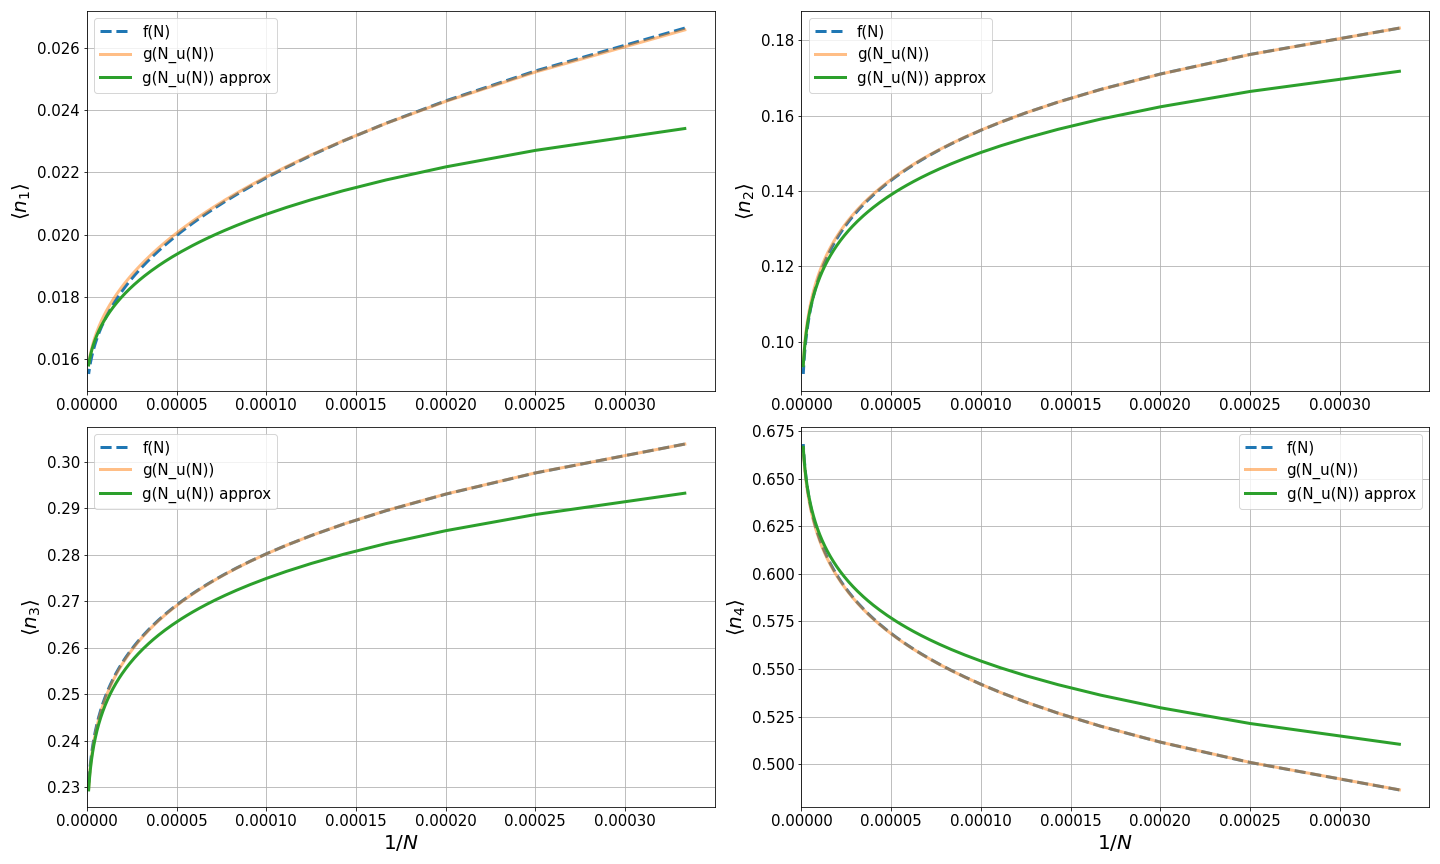
\includegraphics[width=\textwidth]{n_i_fN_vs_gNun.png}
\label{fig:ni_fn_vs_gNun}
\caption{Доли узлов $n_1-n_4$ в линейном масштабе как функции от количества шагов (синий пунктир) \eqref{eq:n_i_log_log}, а так же сложные функции от количества уникальных узлов от количества шагов (оранжевая линия -- прямая подстановка функций  \eqref{eq:gi_appprox2} в \eqref{eq:gi_approx1}, зелёная - аппроксимация \eqref{eq:g_n_expect}), по горизонтали -- обратное количество шагов блуждания $1/N$. Коэффициенты взяты из таблиц \ref{tab:n_i_log_log} и \ref{tab:n_i_u_log_log}.}
\end{figure}

Логарифмический масштаб графиков представлен на рисунке \ref{fig:ni_fn_vs_gNun_log}. 
Здесь ситуация выглядит совершенно иначе: на всех графиках наблюдается расхождение $f_i$ и $g_i$ по мере сближения с нулём.
Причём теперь $g_i$ и её аппроксимация сливаются в одну кривую (что говорит о правильности полученной линеризацией функции \eqref{eq:g_n_expect}). 
Из прошлого раздела мы узнали, что асимпотические пределы $n_1$ и $n_3$ равны в пределах погрешности между выбранными зависимостями.

Однако пределы двух других функций как численно, так и графически расходятся между $f_i$ и $g_i$, что противоречит предположениям о связи зависимостей в пределе бесконечного числа шагов блуждания.


\begin{figure}
\centering
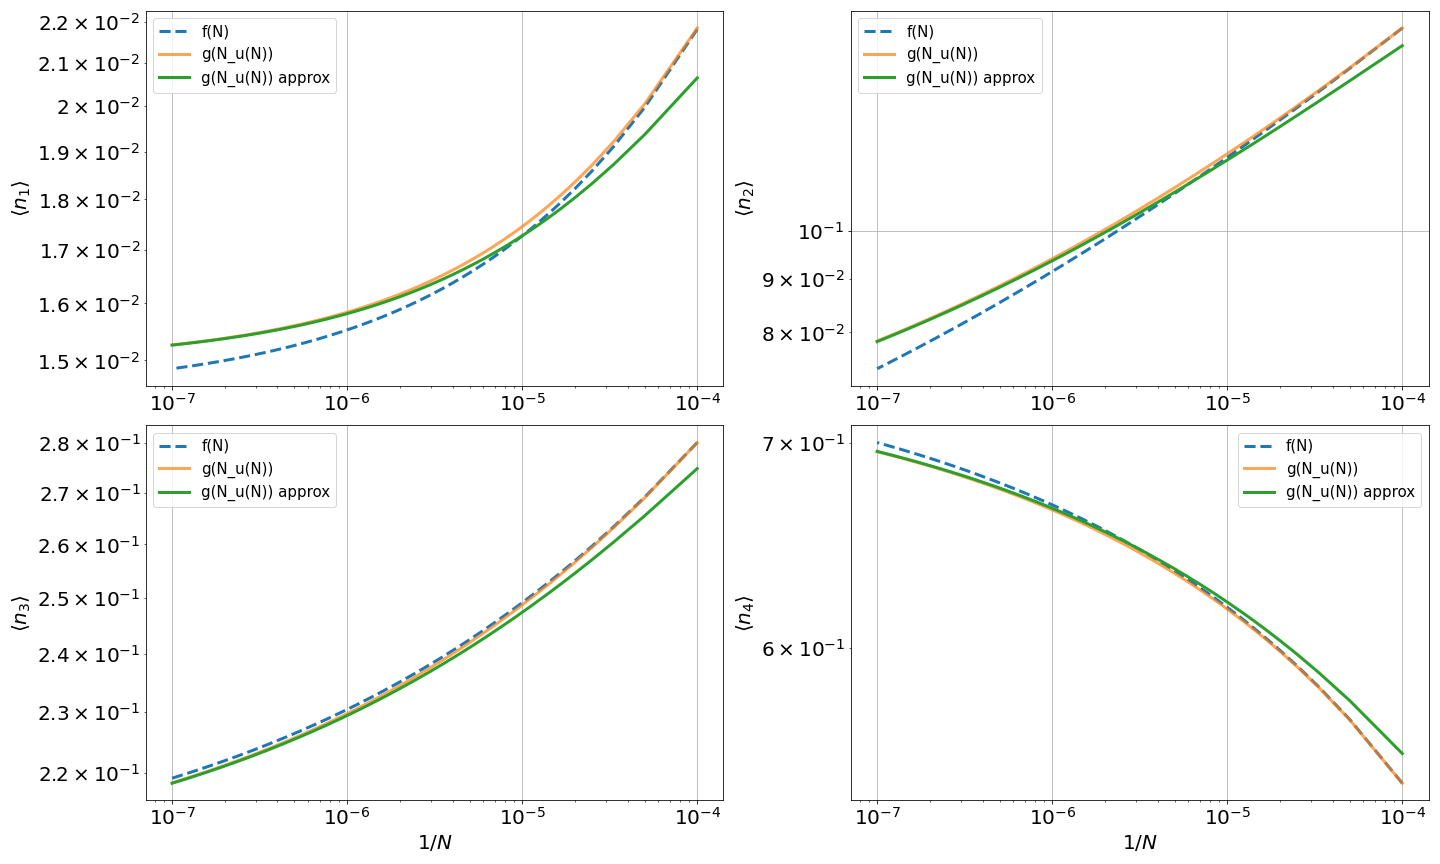
\includegraphics[width=\textwidth]{n_i_fN_vs_gNun_log.png}
\label{fig:ni_fn_vs_gNun_log}
\caption{Доли узлов $n_1-n_4$ в лог-лог масштабе как функции от количества шагов (синий пунктир) \eqref{eq:n_i_log_log}, а так же сложные функции от количества уникальных узлов от количества шагов (оранжевая линия -- прямая подстановка функций  \eqref{eq:gi_appprox2} в \eqref{eq:gi_approx1}, зелёная - аппроксимация \eqref{eq:g_n_expect}), по горизонтали -- обратное количество шагов блуждания $1/N$. Коэффициенты взяты из таблиц \ref{tab:n_i_log_log} и \ref{tab:n_i_u_log_log}.}
\end{figure}